\documentclass{standalone}
\usepackage{tikz}
\usetikzlibrary{decorations.pathmorphing,patterns}

\begin{document}
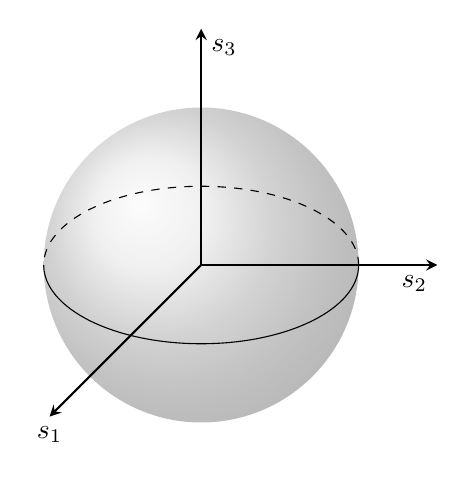
\begin{tikzpicture}
    
    % Ball + equator
    \shade[ball color = gray!40, opacity = 0.4] (0,0) circle (2);
    \draw (-2,0) arc (180:360:2 and 1);
    \draw[dashed] (2,0,0) arc (0:180:2 and 1);
    
    % Axes
    \draw[thick,->, >=stealth] (0,0,0) -- (3,0,0) node[anchor=north east]{$s_2$};
    \draw[thick,->, >=stealth] (0,0,0) -- (0,3,0) node[anchor=north west]{$s_3$};
    \draw[thick,->, >=stealth] (0,0,0) -- (0,0,5) node[anchor=north]{$s_1$};
    
\end{tikzpicture}
\end{document}